\documentclass[12pt]{article}

\usepackage{fullpage}
\usepackage{multicol,multirow}
\usepackage{tabularx}
\usepackage{ulem}
\usepackage[utf8]{inputenc}
\usepackage[russian]{babel}
\usepackage{graphicx}

% Оригиналный шаблон: http://k806.ru/dalabs/da-report-template-2012.tex

\begin{document}

\section*{Лабораторная работа №\,4 по курсу дискрeтного анализа: строковые алгоритмы}

Выполнил студент группы 08-207 МАИ \textit{Дружинин Данила}.

\subsection*{Условие}

\begin{enumerate}
	\item 
	
	Требуется найти все вхождения заданного образца в тексте. Образец и текст представляют собой последовательности элементов некоторого алфавита, при этом текст может быть разбит на строки и слова. Необходимо определить все позиции, с которых начинается полное совпадение образца с подотрезком текста, и для каждого вхождения вывести номер строки и номер слова, соответствующие началу совпадения. Нумерация строк и слов начинается с единицы.
	
	\item Вариант задания: B. 1-2. Алгоритм Кнута–Морриса–Пратта. В качестве алфавита используются целые числа в диапазоне от $0$ до $2^{32}-1$.
\end{enumerate}

\subsection*{Метод решения}

Для решения задачи используется алгоритм Кнута–Морриса–Пратта (КМП), позволяющий находить все вхождения образца в тексте за линейное время. Алгоритм применяется не к строкам, а к последовательностям чисел, однако его логика полностью сохраняется, так как сравнение элементов остаётся операцией равенства.

На первом этапе образец считывается и представляется в виде массива чисел. По этому массиву строится префикс-функция. Для каждой позиции она хранит длину наибольшего собственного префикса образца, совпадающего с суффиксом подмассива, заканчивающегося в данной позиции. Эта информация используется для того, чтобы при несовпадении не возвращаться к началу образца, а продолжать проверку с максимально возможной позиции.

Для построения префикс-функции используется Z-функция. Z-функция вычисляется только для массива образца: значение $z[i]$ равно длине наибольшего префикса образца, совпадающего с подстрокой, начинающейся в позиции $i$. По известным значениям Z-функции префикс-функция восстанавливается за два прохода: сначала для каждого ненулевого $z[i]$ обновляется значение $pf[i + z[i] - 1]$, затем значения распространяются справа налево. После этого вектор Z-функции явно освобождается, и дальнейшая работа ведётся только с префикс-функцией.

После построения префикс-функции осуществляется обработка текста. Текст считывается последовательно, построчно, без сохранения его целиком в памяти. Каждая строка разбивается на отдельные числа (слова), которые обрабатываются по одному. Для каждого текущего элемента текста поддерживается значение переменной, показывающей длину уже совпавшей части образца.

При добавлении нового элемента текста выполняется сравнение с текущим элементом образца. В случае несовпадения происходит переход по префикс-функции к меньшему значению длины совпадения, после чего сравнение повторяется. Если элементы совпадают, длина текущего совпадения увеличивается на единицу.

Когда длина совпадения становится равной длине образца, фиксируется полное вхождение. После этого значение длины совпадения корректируется с помощью префикс-функции для продолжения поиска, что позволяет находить пересекающиеся вхождения.

Для корректного вывода позиции начала каждого вхождения дополнительно используется двусторонняя очередь фиксированного размера, равного длине образца. В неё последовательно добавляются позиции текущих элементов текста (номер строки и номер слова). При превышении размера очереди удаляется самый старый элемент. В момент обнаружения совпадения первый элемент очереди соответствует позиции начала образца в тексте.

Таким образом, алгоритм обрабатывает текст за один проход, не требует дополнительной памяти для хранения всего текста и имеет временную сложность $O(n + m)$, где $n$ — количество элементов текста, а $m$ — длина образца. 

\subsection*{Описание программы}

Программа реализована в виде одного исходного файла на языке C++. Разделение на несколько файлов не используется, так как решение представляет собой компактную реализацию одного алгоритма.

Для хранения позиций элементов текста используется структура:
\begin{itemize}
	\item \texttt{TPosition} — содержит два поля: номер строки (\texttt{Line}) и номер слова в строке (\texttt{Word}).
\end{itemize}

Основные используемые типы данных:
\begin{itemize}
	\item \texttt{std::vector<uint32\_t>} — используется для хранения образца;
	\item \texttt{std::vector<int>} — используется для хранения Z-функции и префикс-функции;
	\item \texttt{std::deque<TPosition>} — используется как скользящее окно фиксированного размера для хранения позиций последних элементов текста;
	\item \texttt{std::string} — используется для чтения строк входного текста;
	\item \texttt{std::istringstream} — используется для разбиения строки на отдельные числа.
\end{itemize}

В программе реализованы следующие функции:
\begin{itemize}
	\item \texttt{ReadPattern} — считывает первую строку входных данных и возвращает образец в виде \texttt{std::vector<uint32\_t>}.
	\item \texttt{BuildZFunction} — вычисляет Z-функцию для заданного массива. Использует оптимизацию на основе Z-блока: при обработке позиции $i$ внутри уже найденного Z-блока $[l, r]$ начальное значение $z[i]$ берётся из зеркальной позиции, что позволяет избежать повторных сравнений. Возвращает вектор значений Z-функции.
	\item \texttt{BuildPrefixFunction} — вычисляет префикс-функцию для образца через Z-функцию. Сначала вызывает \texttt{BuildZFunction} для образца, затем конвертирует результат в префикс-функцию за два прохода. После конвертации вектор Z-функции явно освобождается с помощью \texttt{clear()} и \texttt{shrink\_to\_fit()}.
	\item \texttt{Search} — выполняет потоковый поиск образца в тексте. Принимает образец и префикс-функцию. Построчно считывает текст, поддерживает переменную \texttt{matched} и скользящее окно позиций, выводит координаты каждого найденного вхождения.
	\item \texttt{main} — координирует работу программы: вызывает \texttt{ReadPattern}, \texttt{BuildPrefixFunction} и \texttt{Search}.
\end{itemize}

Архитектура программы линейная: сначала считывается и обрабатывается образец, затем выполняется однопроходный анализ текста с немедленным выводом результатов. Хранение всего текста в памяти не требуется.

\subsection*{Дневник отладки}

В процессе разработки и тестирования программы возникло несколько типичных проблем, связанных с реализацией алгоритма и обработкой входных данных.

\begin{itemize}
	\item \textbf{Ошибка в определении позиции начала совпадения.}  
	Изначально позиция начала вхождения определялась по текущему слову, в котором завершилось совпадение. Это приводило к неверным результатам, так как необходимо было выводить позицию первого элемента образца. Проблема была решена введением скользящего окна (двусторонней очереди), в котором хранятся позиции последних $m$ элементов текста. Начало совпадения определяется как первый элемент этой очереди.
	
	\item \textbf{Некорректная работа при перекрывающихся вхождениях.}  
	На начальном этапе после нахождения совпадения значение текущей длины совпадения обнулялось. Это приводило к пропуску перекрывающихся вхождений. Ошибка была исправлена за счёт использования перехода по префикс-функции (\texttt{matched = pf[matched - 1]}), что соответствует классическому алгоритму КМП.
	
	\item \textbf{Выход за границы массива образца.}  
	В одной из версий кода возникала ситуация, при которой происходило обращение к элементу \texttt{pat[matched]} при \texttt{matched = m}. Это приводило к неопределённому поведению. Проблема была устранена корректным обновлением переменной \texttt{matched} сразу после фиксации совпадения.
	
	\item \textbf{Ошибка при обработке входных данных с ведущими нулями.}  
	На этапе тестирования было замечено, что числа вида \texttt{0011} и \texttt{11} должны считаться одинаковыми. Это было учтено за счёт использования числового типа \texttt{uint32\_t} и стандартного потокового ввода, автоматически приводящего значения к числовому виду.
	
	\item \textbf{Некорректное ограничение размера окна.}  
	Изначально окно позиций не уменьшалось при превышении размера образца, что приводило к накоплению лишних данных и неправильному определению начала совпадения. Проблема была решена удалением самого старого элемента при превышении размера окна.
	
	\item \textbf{Ошибки в нумерации строк и слов.}
	В первых версиях нумерация начиналась с нуля, что противоречило условию задачи. Исправлено путём явной инициализации счётчиков с единицы и корректного обновления значений при переходе к новой строке.

	\item \textbf{Превышение лимита памяти при использовании Z-функции для поиска.}
	В одной из версий Z-функция вычислялась над объединённым массивом \texttt{pat + text}, что является классическим применением Z-алгоритма для поиска. Однако при больших входных данных это потребовало хранения всего текста в памяти, а также вспомогательного массива той же длины, что привело к превышению лимита памяти в 64 МБ. Проблема была решена следующим образом: Z-функция вычисляется только над образцом длиной $m$, по ней восстанавливается префикс-функция, после чего вектор Z-функции явно освобождается. Поиск выполняется потоково с использованием префикс-функции, без хранения текста в памяти. Итоговое потребление памяти составляет $O(m)$ независимо от размера текста.
\end{itemize}

После устранения указанных проблем программа стала корректно обрабатывать все тестовые случаи, включая граничные ситуации и перекрывающиеся вхождения.

\subsection*{Тест производительности}

Для оценки производительности алгоритма была подготовлена отдельная версия программы. Основная реализация алгоритма Кнута--Морриса--Пратта не изменялась: функция построения префикс-функции и цикл поиска были использованы без модификаций.

Для измерения времени выполнения был использован модуль \texttt{std::chrono}. Отдельно измерялось время построения префикс-функции и время выполнения поиска. Чтобы исключить влияние операций ввода-вывода, текст предварительно считывался в память, после чего производился замер только алгоритмической части. Также был отключён вывод найденных вхождений, так как операции вывода существенно влияют на время выполнения.

Во всех экспериментах длина образца фиксировалась и составляла $m = 100$. Размер текста постепенно увеличивался. Были получены следующие результаты:

\begin{center}
	\begin{tabular}{|c|c|}
		\hline
		Количество слов в тексте $n$ & Время поиска, мс \\
		\hline
		100000 & 0.46 \\
		300000 & 1.12 \\
		500000 & 2.61 \\
		1000000 & 3.99 \\
		2000000 & 7.71 \\
		5000000 & 16.99 \\
		\hline
	\end{tabular}
\end{center}

На основе полученных данных был построен график зависимости времени выполнения от размера текста (см. рис.~\ref{fig:kmp}).

\begin{figure}[h]
	\centering
	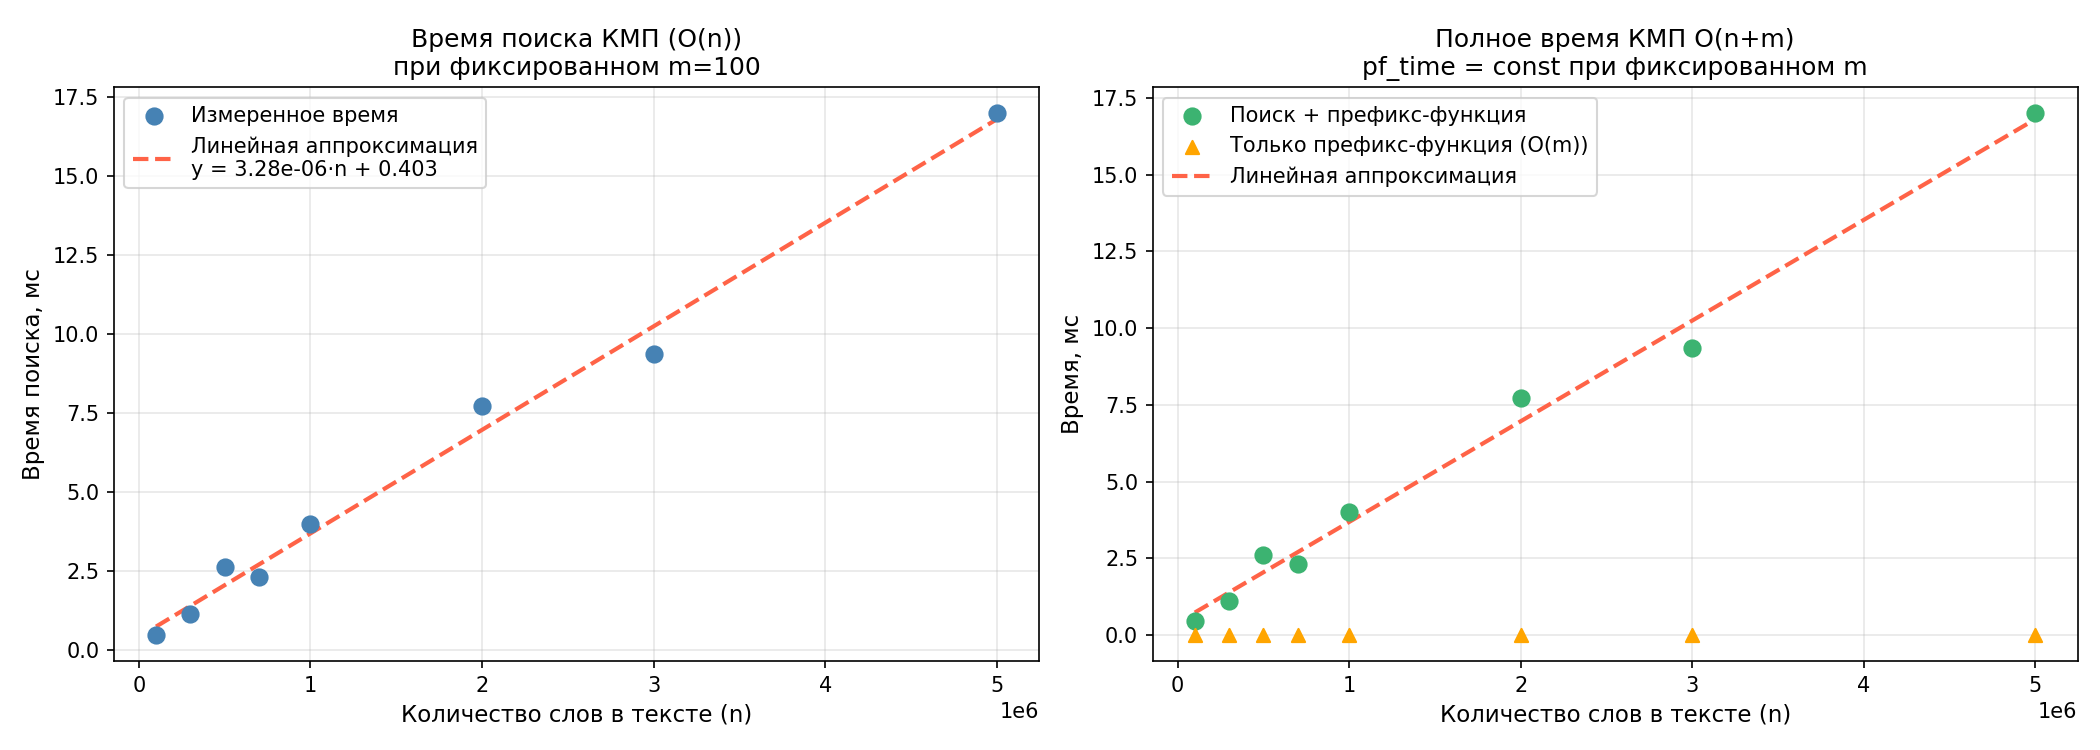
\includegraphics[width=0.9\textwidth]{kmp_performance.png}
	\caption{
		Экспериментальная зависимость времени работы алгоритма Кнута--Морриса--Пратта от размера текста:
		слева показано время поиска при фиксированной длине образца ($m=100$), справа --- полное время работы алгоритма. Видно, что вклад построения префикс-функции практически постоянен.
	}
	\label{fig:kmp}
\end{figure}

Экспериментальные данные хорошо аппроксимируются линейной функцией:
\[
T(n) \approx 3.28 \cdot 10^{-6} n + 0.403.
\]

Это подтверждает линейный рост времени выполнения при увеличении размера входных данных. Незначительные отклонения отдельных точек от аппроксимирующей прямой объясняются погрешностями измерений, особенностями работы кэш-памяти процессора и другими системными факторами.

Отдельно было рассмотрено влияние построения префикс-функции. Так как длина образца фиксирована, время её вычисления практически не зависит от размера текста и остаётся пренебрежимо малым по сравнению с временем поиска.

Таким образом, экспериментальные результаты подтверждают теоретическую оценку сложности алгоритма Кнута--Морриса--Пратта:
\[
O(n + m).
\]

При фиксированном размере образца $m$ сложность сводится к линейной:
\[
O(n).
\]


\subsection*{Недочёты}

Несмотря на корректность реализации алгоритма и соответствие теоретической сложности, в программе остаются некоторые ограничения.

\begin{itemize}
	\item \textbf{Высокая стоимость разбора входных данных.}  
	Текст обрабатывается с использованием \texttt{std::istringstream}, что является достаточно медленным способом парсинга. При очень больших объёмах входных данных именно разбор строк может занимать значительную долю общего времени выполнения. В рамках работы это не оптимизировалось, так как основной целью была реализация алгоритма поиска.
	
	\item \textbf{Дополнительные затраты памяти.}  
	Для определения позиции начала совпадения используется двусторонняя очередь фиксированного размера $m$. Хотя объём используемой памяти невелик, при очень больших значениях $m$ это может приводить к дополнительным накладным расходам.
	
	\item \textbf{Отсутствие оптимизации ввода-вывода.}  
	В основной версии программы используется стандартный ввод и вывод без дополнительной оптимизации (например, отключения синхронизации с \texttt{stdio}). В условиях обработки больших данных это может негативно сказаться на производительности.
	
	\item \textbf{Отсутствие обработки некорректного ввода.}  
	Программа предполагает, что входные данные строго соответствуют формату задачи. Проверка корректности данных (например, наличие нечисловых значений) не выполняется.
	
\end{itemize}

Перечисленные недостатки не влияют на корректность работы алгоритма, однако могут сказываться на производительности и устойчивости программы при работе с нестандартными или экстремально большими входными данными. 

\subsection*{Выводы}

В ходе работы был реализован алгоритм Кнута--Морриса--Пратта для поиска образца в тексте, представленном в виде последовательности чисел. Для построения префикс-функции используется Z-функция, вычисляемая только над образцом, что позволяет сохранить линейную сложность подготовительного этапа при минимальных затратах памяти. Экспериментально подтверждена линейная сложность алгоритма $O(n + m)$, которая при фиксированной длине образца сводится к $O(n)$.

Алгоритм КМП применяется для поиска подстрок и подпоследовательностей в различных типах данных. Типовыми задачами являются поиск фрагментов текста, анализ логов, обработка последовательностей чисел, а также задачи биоинформатики (поиск совпадений в последовательностях ДНК). В данной работе алгоритм был успешно адаптирован для числового алфавита, что демонстрирует его универсальность.

Сложность программирования алгоритма можно оценить как среднюю. Основные трудности связаны с корректной реализацией префикс-функции и обработкой переходов при несовпадениях. Дополнительную сложность представляет необходимость корректного определения позиции начала совпадения, особенно при потоковой обработке текста без хранения всей последовательности в памяти.

В процессе разработки возникали проблемы, связанные с обработкой перекрывающихся вхождений, корректной нумерацией позиций и организацией хранения последних элементов текста. Все указанные трудности были успешно устранены.

Таким образом, реализованный алгоритм является эффективным и универсальным средством поиска, пригодным для обработки больших объёмов данных.

\end{document}

